\documentclass[tikz,border=3pt]{standalone}
\usepackage[utf8]{inputenc}
\usepackage[T1]{fontenc}
\usepackage{lmodern}
\renewcommand{\familydefault}{\sfdefault}
\usepackage{amsmath}
\usepackage{sansmath}\sansmath
\usepackage{pgfplots}\pgfplotsset{compat=1.18,/pgf/number format/use comma,/pgf/number format/1000 sep={.}}
\usetikzlibrary{arrows.meta,calc,positioning,decorations.pathmorphing,patterns}
% paleta del sitio
\definecolor{nar}{HTML}{E8680C}\definecolor{narc}{HTML}{FFB35C}\definecolor{hielo}{HTML}{FFF3E8}
\definecolor{tinta}{HTML}{1D1D1F}\definecolor{gris}{HTML}{6E6E73}\definecolor{lila}{HTML}{7C5CF0}
\definecolor{azul}{HTML}{2F6FD6}\definecolor{menta}{HTML}{17A673}\definecolor{coral}{HTML}{E8342A}
\pgfplotsset{base/.style={axis lines=left,grid=major,grid style={gris!20},tick label style={font=\small},label style={font=\small},axis line style={tinta!80}}}
\begin{document}
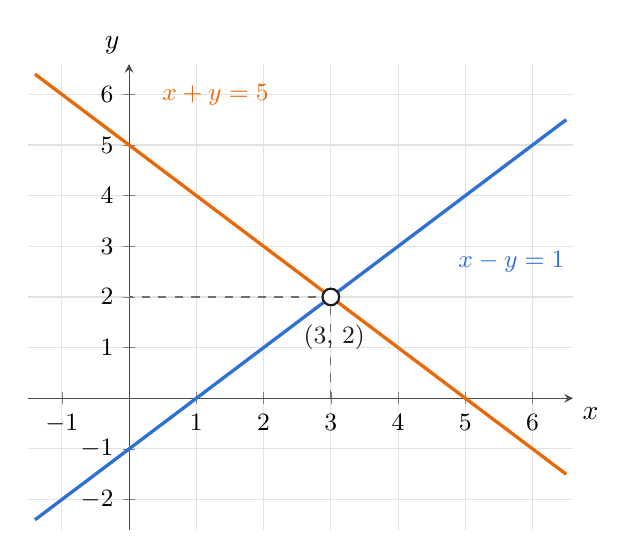
\begin{tikzpicture}
\begin{axis}[base,axis lines=middle,width=8.5cm,height=7.5cm,xmin=-1.5,xmax=6.6,ymin=-2.6,ymax=6.6,xtick={-1,...,6},ytick={-2,...,6},xlabel={$x$},ylabel={$y$},xlabel style={anchor=north west},ylabel style={anchor=south east},clip=false]
\addplot[nar,very thick,domain=-1.4:6.5] {5-x};
\addplot[azul,very thick,domain=-1.4:6.5] {x-1};
\draw[gris,dashed] (axis cs:3,0) -- (axis cs:3,2) -- (axis cs:0,2);
\addplot[only marks,mark=*,mark options={fill=white,draw=tinta,thick},mark size=3pt] coordinates {(3,2)};
\node[tinta,font=\small\bfseries,anchor=north] at (axis cs:3.05,1.65) {$(3,\,2)$};
\node[nar,font=\small\bfseries,anchor=south west] at (axis cs:0.35,5.6) {$x + y = 5$};
\node[azul,font=\small\bfseries,anchor=north west] at (axis cs:4.75,3.1) {$x - y = 1$};
\end{axis}
\end{tikzpicture}
\end{document}
